\documentclass{standalone}
\usepackage{tikz}
\usetikzlibrary{positioning}
\begin{document}

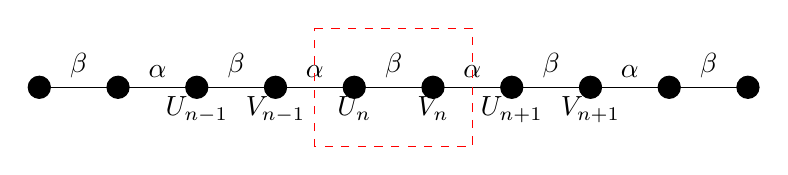
\begin{tikzpicture}
\draw (-4,0) -- (5,0);
\filldraw[black] (-4,0) circle (4pt) node[anchor=north] {};
\filldraw[black] (-3.5,0) circle (0pt) node[anchor=south] {$\beta$};
\filldraw[black] (-3,0) circle (4pt) node[anchor=north] {};
\filldraw[black] (-2.5,0) circle (0pt) node[anchor=south] {$\alpha$};
\filldraw[black] (-2,0) circle (4pt) node[anchor=north] {$U_{n-1}$};
\filldraw[black] (-1.5,0) circle (0pt) node[anchor=south] {$\beta$}; 
\filldraw[black] (-1,0) circle (4pt) node[anchor=north] {$V_{n-1}$};
\filldraw[black] (-0.5,0) circle (0pt) node[anchor=south] {$\alpha$};
\filldraw[black] (0,0) circle (4pt) node[anchor=north] {$U_{n}$};
\filldraw[black] (0.5,0) circle (0pt) node[anchor=south] {$\beta$};
\filldraw[black] (1,0) circle (4pt) node[anchor=north] {$V_{n}$};
\filldraw[black] (1.5,0) circle (0pt) node[anchor=south] {$\alpha$};
\filldraw[black] (2,0) circle (4pt) node[anchor=north] {$U_{n+1}$};
\filldraw[black] (2.5,0) circle (0pt) node[anchor=south] {$\beta$};
\filldraw[black] (3,0) circle (4pt) node[anchor=north] {$V_{n+1}$};
\filldraw[black] (3.5,0) circle (0pt) node[anchor=south] {$\alpha$};
\filldraw[black] (4,0) circle (4pt) node[anchor=north] {};
\filldraw[black] (4.5,0) circle (0pt) node[anchor=south] {$\beta$};
\filldraw[black] (5,0) circle (4pt) node[anchor=north] {};
\draw[red, dashed] (-0.5,0.75) -- (1.5, 0.75) -- (1.5, -0.75) -- (-0.5, -0.75) -- cycle;
\end{tikzpicture}



\end{document}